% !TEX TS-program = xelatex
% !TEX encoding = UTF-8 Unicode
% !Mode:: "TeX:UTF-8"
\documentclass[bachelor,nocolorlinks, printoneside]{seuthesis} % 本科
% \documentclass[master]{seuthesis} % 硕士
% \documentclass[doctor]{seuthesis} % 博士
% \documentclass[engineering]{seuthesis} % 工程硕士
\usepackage{CJK,CJKnumb}
\usepackage{amsmath}
\usepackage{amsfonts} 
\usepackage{bm} 
\usepackage{algorithm}
\usepackage{algorithmicx}
\usepackage{algpseudocode}
\usepackage{subfigure}

\floatname{algorithm}{算法}
\renewcommand{\algorithmicrequire}{\textbf{输入:}}
\renewcommand{\algorithmicensure}{\textbf{输出:}}
 % 这里是导言区

\begin{document}

%# -*- coding: utf-8-unix -*-
\categorynumber{000} % 分类采用《中国图书资料分类法》
\UDC{000}            %《国际十进分类法UDC》的类号
\secretlevel{公开}    %学位论文密级分为"公开"、"内部"、"秘密"和"机密"四种
\studentid{09015131}   %学号要完整,前面的零不能省略。

\title{集群缓存系统负载均衡算法的设计与实现}{}{CW-Cache: Column-wise Load Balancing for Structured Data}{}
\author{郑云川}{Yunchuan Zheng}
\advisor{肖卿俊}{副教授}{Qingjun Xiao}{Associate Prof.}
\coadvisor{王威}{助理教授}{Wei Wang}{Assistant Prof.}

% \degree{工学硕士} % 详细学位名称
\major[12em]{计算机科学与技术}
\defenddate{答辩日期}
\authorizedate{学位授予日期}
\department{计算机科学与工程}{Computer Science and Engineering}
\duration{2018年12月—2019年6月}
\address{HKUST}
% \thanks{本论文获国家XXX计划项目(2012AA00A00)和国家杰出青年科学基金项目(01234567)资助。}

\maketitle

%# -*- coding: utf-8-unix -*-
%%==================================================
%% abstract.tex for seuthesis Bachelor Thesis
%%==================================================

\begin{abstract}{希腊字母,腓尼基字母,语言,深度学习}
    希腊字母源自腓尼基字母。腓尼基字母只有辅音,从右向左写。希腊语的元音发达,希腊人增添了元音字母。因为希腊人的书写工具是蜡板,有时前一行从右向左写完后顺势就从左向右写,变成所谓“耕地”式书写,后来逐渐演变成全部从左向右写。字母的方向也颠倒了。罗马人引进希腊字母,略微改变变为拉丁字母,在世界广为流行。希腊字母广泛应用到学术领域,如数学等。
    
    希腊字母是希腊语所使用的字母,是世界上最早的有元音的字母,也广泛使用于数学、物理、生物、天文等学科。俄语等使用的西里尔字母也是由希腊字母演变而成。希腊字母进入了许多语言的词汇中,英语单字“alphabet”(字母表),源自拉丁语“alphabetum”,源自希腊语“αλφαβητον”,即为前两个希腊字母α(“Alpha”)及β(“Beta”)所合成,三角洲(“Delta”)这个词就来自希腊字母Δ,因为Δ是三角形。
    \end{abstract}
    
    \begin{englishabstract}{Greek Alphabet, Phoenician Alphabet, Language, Deep Learning}
    The Greek alphabet has been used to write the Greek language since the late 9th century BC or early 8th century BC It was derived from the earlier Phoenician alphabet, and was the first alphabetic script to have distinct letters for vowels as well as consonants. It is the ancestor of the Latin and Cyrillic scripts.Apart from its use in writing the Greek language, in both its ancient and its modern forms, the Greek alphabet today also serves as a source of technical symbols and labels in many domains of mathematics, science and other fields.
    
    In its classical and modern forms, the alphabet has 24 letters, ordered from alpha to omega. Like Latin and Cyrillic, Greek originally had only a single form of each letter; it developed the letter case distinction between upper-case and lower-case forms in parallel with Latin during the modern era.
    \end{englishabstract}


\tableofcontents

% \begin{terminology}
% \begin{table}[h]
% \renewcommand\arraystretch{1.5}
% %\Large
% \begin{tabular}{>{\LARGE}m{0.2\textwidth} <{\centering}m{0.7\textwidth}}
% a & 如同汉字起源于象形,拉丁字母表中的每个字母一开始都是描摹某种动物或物体形状的图画\\

% b&和A一样,字母B也可以追溯到古代腓尼基。在腓尼基字母表中B叫beth,代表房屋,在希伯来语中B也叫beth,也含房屋之意。\\

% c& 字母C在腓尼基人的文字中叫gimel,代表骆驼。它在字母表中的排列顺序和希腊字母Γ(gamma)相同,实际上其字形是从后者演变而来的。C在罗马数字中表示100。\\

% d&D在古时是描摹拱门或门的形状而成的象形符号,在古代腓尼基语和希伯来语中叫做daleth,是“门”的意思,相当于希腊字母Δ(delta)。\\

% \end{tabular}
% %\caption{my table}
% \end{table}
% \end{terminology}


\begin{Main} % 开始正文

%# -*- coding: utf-8-unix -*-
%%==================================================
%% introduction.tex for seuthesis Bachelor Thesis
%%==================================================

\chapter{绪论}
\label{chp:intro}

本章是课题的绪论部分。在此章中,我们首先介绍了课题的实际背景,接下来说明了课题的目的和意义,并且对当前的研究现状做了简要的调研与分析,最后介绍了课题的主要研究内容。

\section{课题背景}

\subsection{大数据}

\par 因为技术的不断发展,包括物联网,云计算的崛起\cite{botta2016integration}、智能设备的流行等,在当今时代各种各样不同的领域(例如健康领域、政府、社交网络、营销、财务),每一天都在以前所未有的速度产生大量的数据\cite{oussous2018big}。从海量的数据中,我们能够挖掘出大量有用的规律,对人们的生活产生积极的影响。在大数据革命之前,大公司很难将他们的数据存档保存较长时间,也难以管理庞大的数据集。传统技术存储能力有限,管理工具很昂贵,它们缺乏大数据背景所需要的灵活性、可扩展性和性能。事实上,大数据管理需要大量资源,新方法和强大技术,进一步来说,大数据需要清洗,处理,分析,保护数据,并提供对大量不断发展的数据集的细粒度访问\cite{oussous2018big}。为了应对大数据带来的机遇和挑战,学界和业界开展了大量的研究与开发工作,发展出来众多技术,提供了很多成熟的模型、框架、软件。典型的互联网大数据平台(如图~\ref{fig:frame})从上至下大致可分为三个部分:

\begin{itemize}
	\item 数据采集:将应用程序产生的数据和日志等同步到大数据系统,同步时数据可能还需经过清洗、转化等过程;
	\item 数据处理:包括大数据存储、离线计算和流式计算等;
	\item 数据输出与展示:大数据经过处理后将有价值的信息存入数据库,通过数据库给用户提供所需信息,或者给运营、决策人员提供所需信息。
\end{itemize}

\par 此外,将三个部分整合起来的是大数据任务调度管理系统,它会管理数据的同步、集群资源的分配等等。
\begin{figure}[ht]
	\centering
	\includegraphics[width=0.50\paperwidth]{img/introduction/big-data-framework.png}
	\caption{典型的互联网大数据平台架构。}
	\label{fig:frame}
	%\vspace{-.15in}
\end{figure}

% \subsection{内存缓存}
% \par 在大数据平台中(图~\ref{fig:frame}),数据处理是非常重要的一环,实现对数据的高效清洗、存储和挖掘是这个环节的目标。对计算能力的需求随着数据量的急剧增加而增加,但是单机的处理能力和 I/O 性能并没有跟上这种增长,越来越多的企业不得不向外扩展他们的计算至集群模式\cite{Zaharia:2016:AFG:3002856}。集群环境对编程平台提出了更高的要求,主要有三方面,一是程序需要并行化执行,二是需要强大的容错能力,三是动态地扩展和缩减计算资源,为此,越来越多的编程模型被设计出来。在存储方面,谷歌提出了分布式文件系统GFS(Google File System)\cite{51},对应的开源实现是HDFS(Hadoop File System)\cite{hdfs},它实现了对成千上万台机器上的大规模数据进行高效地存储、访问,并且具有高度容错能力。计算框架方面,起初,谷歌的 MapReduce\cite{dean2008mapreduce}提出了一种简单通用而且能够自动处理故障的批处理计算模型,但是它将中间以及最终结果保存在磁盘上,消耗大量I/O时间,不利于重用计算结果。Spark\cite{Zaharia:2016:AFG:3002856}、Pregel\cite{malewicz2010pregel}等采用内存计算方案来加速计算,实现数据的重复利用。很多系统的性能瓶颈主要是I/O,包括磁盘读写和网络远程读写的延迟,为了进一步提高性能,一种典型的方法是部署缓存,并且将数据在分布式集群中服务器的内存进行缓存\cite{ananthanarayanan2012pacman},并且尽力实现计算任务和数据的本地性(locality)。内存的读写速度远高于磁盘,将计算与数据部署在相同的机器也能节约网络开销。
\par 在大数据平台中(图~\ref{fig:frame}),数据处理是非常重要的一环,实现对数据的高效清洗、存储和挖掘是这个环节的目标。对计算能力的需求随着数据量的急剧增加而增加,但是单机的处理能力和 I/O 性能并没有跟上这种增长,越来越多的企业不得不向外扩展他们的计算至集群模式\cite{Zaharia:2016:AFG:3002856}。集群环境对编程平台提出了更高的要求,主要有三方面,一是程序需要并行化执行,二是需要强大的容错能力,三是动态地扩展和缩减计算资源,为此,越来越多的编程模型被设计出来。在存储方面,谷歌提出了分布式文件系统GFS(Google File System)\cite{51},对应的开源实现是HDFS(Hadoop File System)\cite{hdfs},它实现了对成千上万台机器上的大规模数据进行高效地存储、访问,并且具有高度容错能力。计算框架方面,起初,谷歌的 MapReduce\cite{dean2008mapreduce}提出了一种简单通用而且能够自动处理故障的批处理计算模型,但是它将中间以及最终结果保存在磁盘上,消耗大量I/O时间,不利于重用计算结果。Spark\cite{Zaharia:2016:AFG:3002856}、Pregel\cite{malewicz2010pregel}等采用内存计算方案来加速计算,实现数据的重复利用。

\subsection{集群缓存}
\par 由于近年来数据中心架构的改进~\cite{singh2015jupiter} 和高速网络设备的出现\cite{huawei_nuwa,asanovic2014firebox,alistarh15a},网络带宽和存储器I/O带宽之间的差距正在迅速减小~\cite{latency_trends,p802_3ba,Han13a,Gao16a},因此,云计算系统的性能瓶颈正迅速从网络转变为存储器I/O。先前的工作证明从本地硬盘读取数据相比网络远程读取并没有显著的优势 ~\cite{Ananthanarayanan11a},这个结论同样适用于固态硬盘(SSD)。最近的一个研究~\cite{Jonas17a} 表明将数据存储在EC2实例的一个本地SSD上甚至比把数据写到Amazon S3 ~\cite{amazons3}上还要慢,Amazon S3是一个远程的提供了PUT/GET接口的对象存储服务。当磁盘本地化变得无关紧要,云端对象存储如 Amazon S3~\cite{amazons3}、 Windows Azure Storage~\cite{azure_storage}、和OpenStack Swift~\cite{swift}等,逐渐取代与计算同地的存储(尤其是HDFS~\cite{shvachko2010hadoop}),作为数据密集型应用的首选存储方式。

\par 然而,云端对象存储在磁盘I/O上依然是瓶颈~\cite{rashmi2016ec},因为从磁盘读数据比从内存读数据慢至少两个数量级,考虑到这个问题,集群缓存系统,例如Alluxio~\cite{alluxio}、Memcached~\cite{memcached}和Redis~\cite{redis},被越来越多的云端对象存储系统部署来提供内存速度级别的低延迟数据访问,而集群缓存系统面对的一个很大的挑战便是如何实现负载均衡。

\par 一个能够实现分布式内存缓存的系统是Alluxio。Alluxio\cite{li2014tachyon}是开源的分布式内存文件系统,旨在作为上层繁多的计算框架(如MapReduce、Apache Spark、Apache Storm、Apche Mahout等)与底层存储层(如文件系统、对象存储、键值对存储等)的中间层,提供统一的文件读写的接口,实现全局的数据访问、高效的内存数据共享、跨应用的数据管理、高效的网络带宽利用,它借助“血缘关系”、检查点机制提供强大的容错能力。鉴于这些特点,alluxio也非常适合作为内存缓存系统,进一步加速数据分析应用。


\subsection{负载均衡}
\par 上一小节提及的Apache Spark等内存计算方案的一个重要挑战是负载不均,在先前工作 
\cite{ananthanarayanan2011scarlett,rashmi2016ec} 中,研究人员已经发现了生产集群中负载不均的两个来源:\emph{文件热门程度倾斜} 和 \emph{网络流量不均}。

\par 在数据中心中,我们普遍观察到,文件(数据对象)热门程度存在倾斜,并且遵循Zipf分布~\cite{rashmi2016ec, ananthanarayanan2011scarlett, ananthanarayanan2012pacman, li2014tachyon},也就是说,数据访问的大部分请求是由一小部分非常热门的文件贡献的。图~\ref{fig:Yahoo_trace}描述了Yahoo!集群查询数据集~\cite{yahoo!_trace}中文件的热门程度和文件大小的分布,从这个数据集可以得到某两个月内对超过四千万个文件的访问的统计数据。我们发现绝大多数文件($\sim 78\%$)存储的是冷门数据,很少被访问($<10$ times),只有 $2\%$ 的文件有高访问量($\ge100$),这些文件通常比那些冷门的文件大很多($15$-$30 \times$)。由于这些文件较大的体积和较高的访问量,缓存这些文件的服务器很容易负荷过重。

\begin{figure}[t]
\centering
   \includegraphics[width=0.7\textwidth]{img/introduction/Yahoo_pop-eps-converted-to.pdf}
   \caption{Yahoo!集群上观察到的文件热门程度(蓝色)和文件大小(橙色)的分布~\cite{yahoo!_trace}.}
\label{fig:Yahoo_trace}
\vspace{-.1in}
\end{figure}

\par 这个问题由于网络负载不均而加重,这在生产环境的数据中心非常普遍~\cite{Kandula09a,Chowdhury13a,Greenberg09a,rashmi2016ec},例如,在研究~\cite{rashmi2016ec}中,研究者测量了Facebook一个集群所有上行和下行链路中最大利用率和平均利用率的比值,结果表明这个比值在半数以上的时间里保持在4.5以上,这意味着严重的负载不均。在SP-Cache~\cite{Yu:2018:SLR:3291656.3291658}的研究中,研究人员分别测量了在有无内存缓存的情况下,不同请求速率下的文件的平均读延迟,结果表明~\ref{fig:impact_of_imbalance}当集群负载不重时(每秒$5$个请求),内存缓存带来了显著性好处,降低平均读延迟达 $5\times$,然而,当负载骤然增大,集群中的热点机器变得突出,缓存带来的好处迅速减少,尤其当请求速率大于$9$,读延迟就由热点服务器的网络拥塞决定,内存缓存就变得\emph{无关紧要}。

\begin{figure}[t]
    \centering
    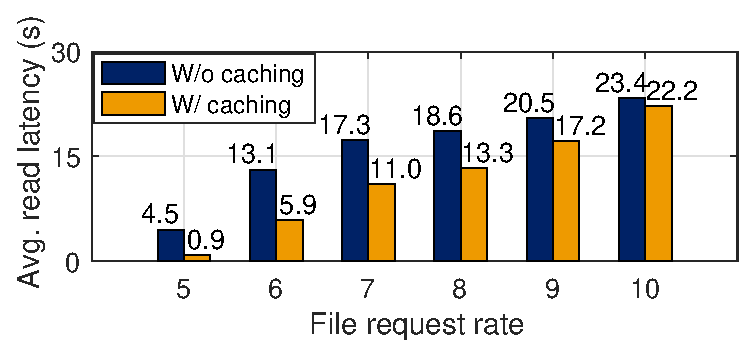
\includegraphics[width=0.8\textwidth]{img/introduction/latencies_under_imbalance}
    \caption{有/无缓存的情况下平均读延迟随着负载增加而增加。}
    \label{fig:impact_of_imbalance}
    \vspace{-.15in}
\end{figure}

\section{研究现状}

\par 当今的数据并行集群依赖内存计算方案来进行高性能的数据分析工作\cite{li2014tachyon, presto, Zaharia:2016:AFG:3002856, power2010piccolo, memcached, memsql},通过将数据对象缓存在内存中, I/O 密集型应用相对于传统的磁盘解决方案能够获得数量级的性能提升\cite{li2014tachyon, Zaharia:2016:AFG:3002856, power2010piccolo}

\par 然而,内存计算方案面对的一个严峻的挑战是缓存服务器之间严重的负载不均衡。在生产集群中,数据对象有严重的热门程倾斜,这意味着对一小部分非常热门的文件访问占据了总访问的很大一部分\cite{rashmi2016ec, ananthanarayanan2011scarlett, ananthanarayanan2012pacman}。存储有热门文件的缓存服务器因此变为访问热点,这个问题因为网络的负载不均衡而进一步恶化。据报道,在 Facebook 的一个集群中,负载最重的链路的利用率在 $50\%$ 的时间里比平均链路利用率高出 4.5 倍\cite{rashmi2016ec}。访问热点和网络负载不均导致了 I/O 性能极大下降,这甚至可能会抵消内存计算带来的性能提升。

\par 因此,保证负载均衡是提高集群缓存性能的关键,这方面的解决方案包括选择性复制\cite{ananthanarayanan2011scarlett}、纠删码\cite{rashmi2016ec}和选择分割\cite{Yu:2018:SLR:3291656.3291658},前二者是借助缓存冗余来减缓访问热点机器的负担,第三个是根据文件的热门程度将文件分割成不同份数,并随机放置在不同服务器上,分散请求负载。

\subsection{选择复制}

\par 选择复制方案基于文件的热门程度对文件进行复制~\cite{ananthanarayanan2011scarlett,hong2013understanding},也就是说,一个文件的访问频率越高,它会越多被复制,并分散在集群中,一个文件的读请求就能随机选择一台含有这个文件副本的服务器提供服务。这样,读请求的负载就被均匀分散,提高负载均衡。

\par 虽然选择复制已被证明对于基于磁盘的存储系统是有效的~\cite{ananthanarayanan2011scarlett},但是因为复制带来了高额的内存开销,它在集群缓存上表现不佳~\cite{huang2014characterizing,rashmi2016ec}。研究~\cite{Yu:2018:SLR:3291656.3291658}的实验得出,内存开销的 \emph{线性增加}(热门文件副本数增加)换来了读延迟的 \emph{亚线性降低},而且热门文件的体积通常比较大(图~\ref{fig:Yahoo_trace})。

\subsection{纠删码}

\par 有研究利用\emph{纠删码}~\cite{huang2012erasure,sathiamoorthy2013xoring} 来实现缓存服务器之间的负载均衡且避免产生高额的内存开销。一个$(k,n)$的纠删码方案能够将一个文件均匀地切分成$k$份,然后计算同样大小的$n-k$个 \emph{奇偶校验分区},原始文件能通过解码$n$份中的任意$k$份来获得,从而使得读请求的负载被分散到$n$台服务器上。内存的额外开销是$(n-k)/k$,在实际设定中比选择复制低(至少 $1\times$)。
\par 这个方法的一个有效实现是EC-Cache~\cite{rashmi2016ec},它在读取文件时通过\emph{迟绑定}来减轻落后机器的影响,换句话说,EC-Cache随机读取文件分区中的$k+1$份,等待其中的$k$份完成读取,而不是恰好读取$k$份。EC-Cache在读文件的中位和尾延迟都比选择复制低很多~\cite{rashmi2016ec}。然而,EC-Cache在读(写)时带来巨大的解码(编码)的额外开销,即使有高度优化的编码和实现方案,解码的开销仍会对读请求产生高达$30\%$~\cite{rashmi2016ec}延迟。

\subsection{选择分割}

\par 研究~\cite{Yu:2018:SLR:3291656.3291658}中提出了SP-Cache来实现集群缓存的负载均衡,同时避免高额的内存和计算开销。它选择性地将热门文件根据其大小和热门程度,分割成一定数目的文件分区,随机缓存到不同的缓存服务器上,这样分散了读请求的负载,同时读操作可以并行,提升性能。SP-Cache建立了一个上限分析来量化平均延迟~\cite{Yu:2018:SLR:3291656.3291658},并基于这个推导设计了一个高效的算法来决定每个文件的最佳分区数量,文件分割的数目太小则不足以缓解热点机器的压力,分割的数目太大则容易受到慢机器的影响。此外它采集一段时间内集群中文件的访问数据,周期性地调整各个文件的分区数目。选择分割在不产生高额内存和计算开销的情况下实现可负载均衡,但因为其分割的特性,缓存无冗余,容错性依赖底层文件系统,且读取文件必须读取所有分区,会受到慢机器的影响。

\subsection{更细粒度负载均衡}

\par 以上方案都是针对一般意义上的文件来考虑负载均衡的,优点是非常通用,毋需考虑文件的语义,对于任何格式的文件都可以使用。它们负载均衡的粒度是文件,那么问题来了,能否在更细的粒度进行负载均衡,提高缓存效率呢?对于语义清晰的结构化数据,比如Parquet文件~\cite{parquet},如果在文件的内部列与列存在热门程度倾斜,列之间被共同查询的概率也存在倾斜,那么就没有必要去分割或者复制整个文件,只要对一个文件热门的这一部分,例如其中一列或者多列进行复制或者分割就行。这样能够节约内存,提高使用效率,因为内存总是有限的,而且一部分内存需要给计算任务使用,那么留作缓存的就更少了。这个目标的挑战在于底层分布式文件系统需要了解文件的语义,与上层的应用通信来获得这部分信息,可能产生一定程度的耦合,同时我们需要明智地决定对文件的哪些列进行复制或分割,在哪些机器上进行缓存。

\section{研究的目的与内容}
当前的大数据系统主要采用复制的方式来进行容错和负载均衡,而服务器内存的容量往往有限,缓存会产生不可忽视的内存开销。根据本项目的前期调研,生产集群中结构化数据(数据表)的不同列之间,热门程度(被访问热度)存在倾斜,列与列之间共同被查询的概率也存在倾斜,我们希望复制数据表中比较热门的列,而不是全表,并基于列与列之间被共同查询的概率设计一定的放置策略,实现以更少的内存,来获得相似的负载均衡效果的目标,从而节约资源,提高缓存效率。

总的来说,本课题的主要研究内容是上文提出的针对结构化数据文件的更细粒度(列级别)的负载均衡方案,具体来说:

\begin{itemize}
	\item 利用具有代表性的基准查询数据集,如TPC-DS, TPC-H等,测量数据表中列之间的查询频率,以及列与列之间被共同查询的频率,分析其中的统计及其他客观规律,为本项目的可行性奠定理论基础。
	\item 通过实验探究SQL查询过程中,数据的shuffle过程对任务执行时间的影响,证明数据表中相关列“捆绑放置”(bundle)的有效性,进一步强化项目的理论基础。
	\item 搭建Spark SQL~\cite{armbrust2015spark},Alluxio~\cite{alluxio},HDFS~\cite{shvachko2010hadoop}为主的集群系统,探索各组件之间通信协作机制,为项目方案实现奠定基础。
	\item 基于已有条件,主要在Alluxio~\cite{alluxio}基础上添加模块,使得Alluxio能够获取热门度以及关联性等信息,查阅相关文献,设计实现细粒度的负载均衡算法,并在AWS EC2搭建实验环境,进行测试。
\end{itemize}

\section{论文结构}

\par 本文一共七章,下面分别介绍每一章的主要内容。%\show \baselineskip

\par 第一章是绪论,主要介绍了本研究课题的背景,集群缓存与负载均衡的现状,接着对当前最新的研究进展做了简介,最后提及此课题的研究目的和主要内容。

\par 第二章是研究动机,用三个实验分别探究列的访问热度倾斜规律,数据表内部的shuffling和shuffling的影响,为课题进行提供基础。

\par 第三章是Column-aware方案与缺点,介绍了一个易想到的直接的方案,然后分析了我们现有的条件,指出此方案的确定和不实用,为我们的正式方案提供参考。

\par 第四章是CW-Cache:设计与分析,这一章我们提出采用Bundle-K方案的CW-Cache系统,并进行数学建模与仿真实验,论证以列的热度信息估算列的共同访问模式,最终求出最优的复制的列数$K$ 和复制的份数 $r$的可行性。

\par 第五章是实现,介绍了CW-Cache系统的框架,各部分的细节以及系统的额外开销。

\par 第六章是测试与评估,从任务执行时间和负载均衡程度来评估我们所实现的CW-Cache系统。

\par 第七章是总结与展望,此章总结了本项目完成的不足,提出CW-Cache存在的缺陷,指出未来的研究工作应该改进完善的地方。


\end{Main} % 结束正文

\begin{Acknowledgement}{}
    这次的毕业论文设计总结是在我的指导老师xxx老师亲切关怀和悉心指导下完成的。从毕业设计选题到设计完成,x老师给予了我耐心指导与细心关怀,有了莫老师耐心指导与细心关怀我才不会在设计的过程中迷失方向,失去前进动力。x老师有严肃的科学态度,严谨的治学精神和精益求精的工作作风,这些都是我所需要学习的,感谢x老师给予了我这样一个学习机会,谢谢!
    
      感谢与我并肩作战的舍友与同学们,感谢关心我支持我的朋友们,感谢学校领导、老师们,感谢你们给予我的帮助与关怀;感谢肇庆学院,特别感谢计算机科学与软件学院四年来为我提供的良好学习环境,谢谢!
\end{Acknowledgement}

% 参考文献
\bibliography{seuthesis}



\newpage
\printindex % 索引

%\begin{thebibliography}{99}


%\bibliographystyle{ieee}
%\bibliography{seuthesis}


\end{document}
